\section{Strategy}
\begin{figure}[H]
	\centering
	\textbf{High level workflow}
	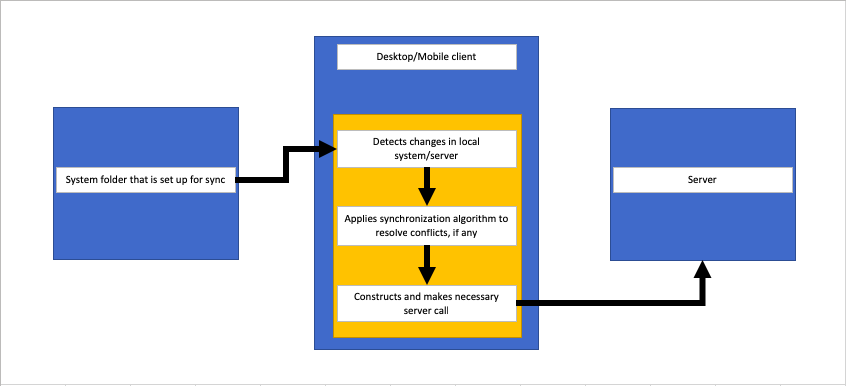
\includegraphics[width=\linewidth]{images/1.png}
	\caption{Flow of control between client and server}
\end{figure}\par
In our Agile workflow, we will start by building a basic prototype of the desktop client. This prototype will perform functionalities of Create, Edit, Rename and Delete for non-conflicting files for single user. It will also have a \emph{Upload} and \emph{Download} button to manually invoke synchronization. Then we will extend this prototype to handle conflict scenarios. The potential conflict scenarios and their resolution are stated in table 1.\newline

Once the conflict resolution algorithm implementation is stable, we will develop the mobile client prototype followed by testing conflict resolution using mobile-desktop client pair. After satisfactory testing, we will move to the final phase of introducing automatic file sync using \emph{file system notification} and \emph{server polling}. Note: We are still contemplating on whether automatic sync should be a desktop-only feature due to constraints on mobile such as battery-life, available internet allowance etc.

\begin{itemize}
\item \textbf{Milestone 1}: Prototype of desktop client for single user with manual sync.
\item \textbf{Milestone 2}: Prototype of conflict resolution on desktop client for multiple users with manual sync.
\item \textbf{Milestone 3}: Prototype of mobile client for multiple users with manual sync.
\item \textbf{Milestone 4}: Enable automatic sync on desktop client.
\end{itemize}
